\chapter{SM}
Følgende afsnit beskriver SM'ens hardware i de enkelte blokke, grænsefladerne derimellem samt funktionen af blokkene.

\section{Overordnet design}
Nedenfor ses det overordnede hardware blokdiagram. Herefter følger en beskrivelse af de forskellige blokke samt signaler.
\begin{figure}[H]
\centering
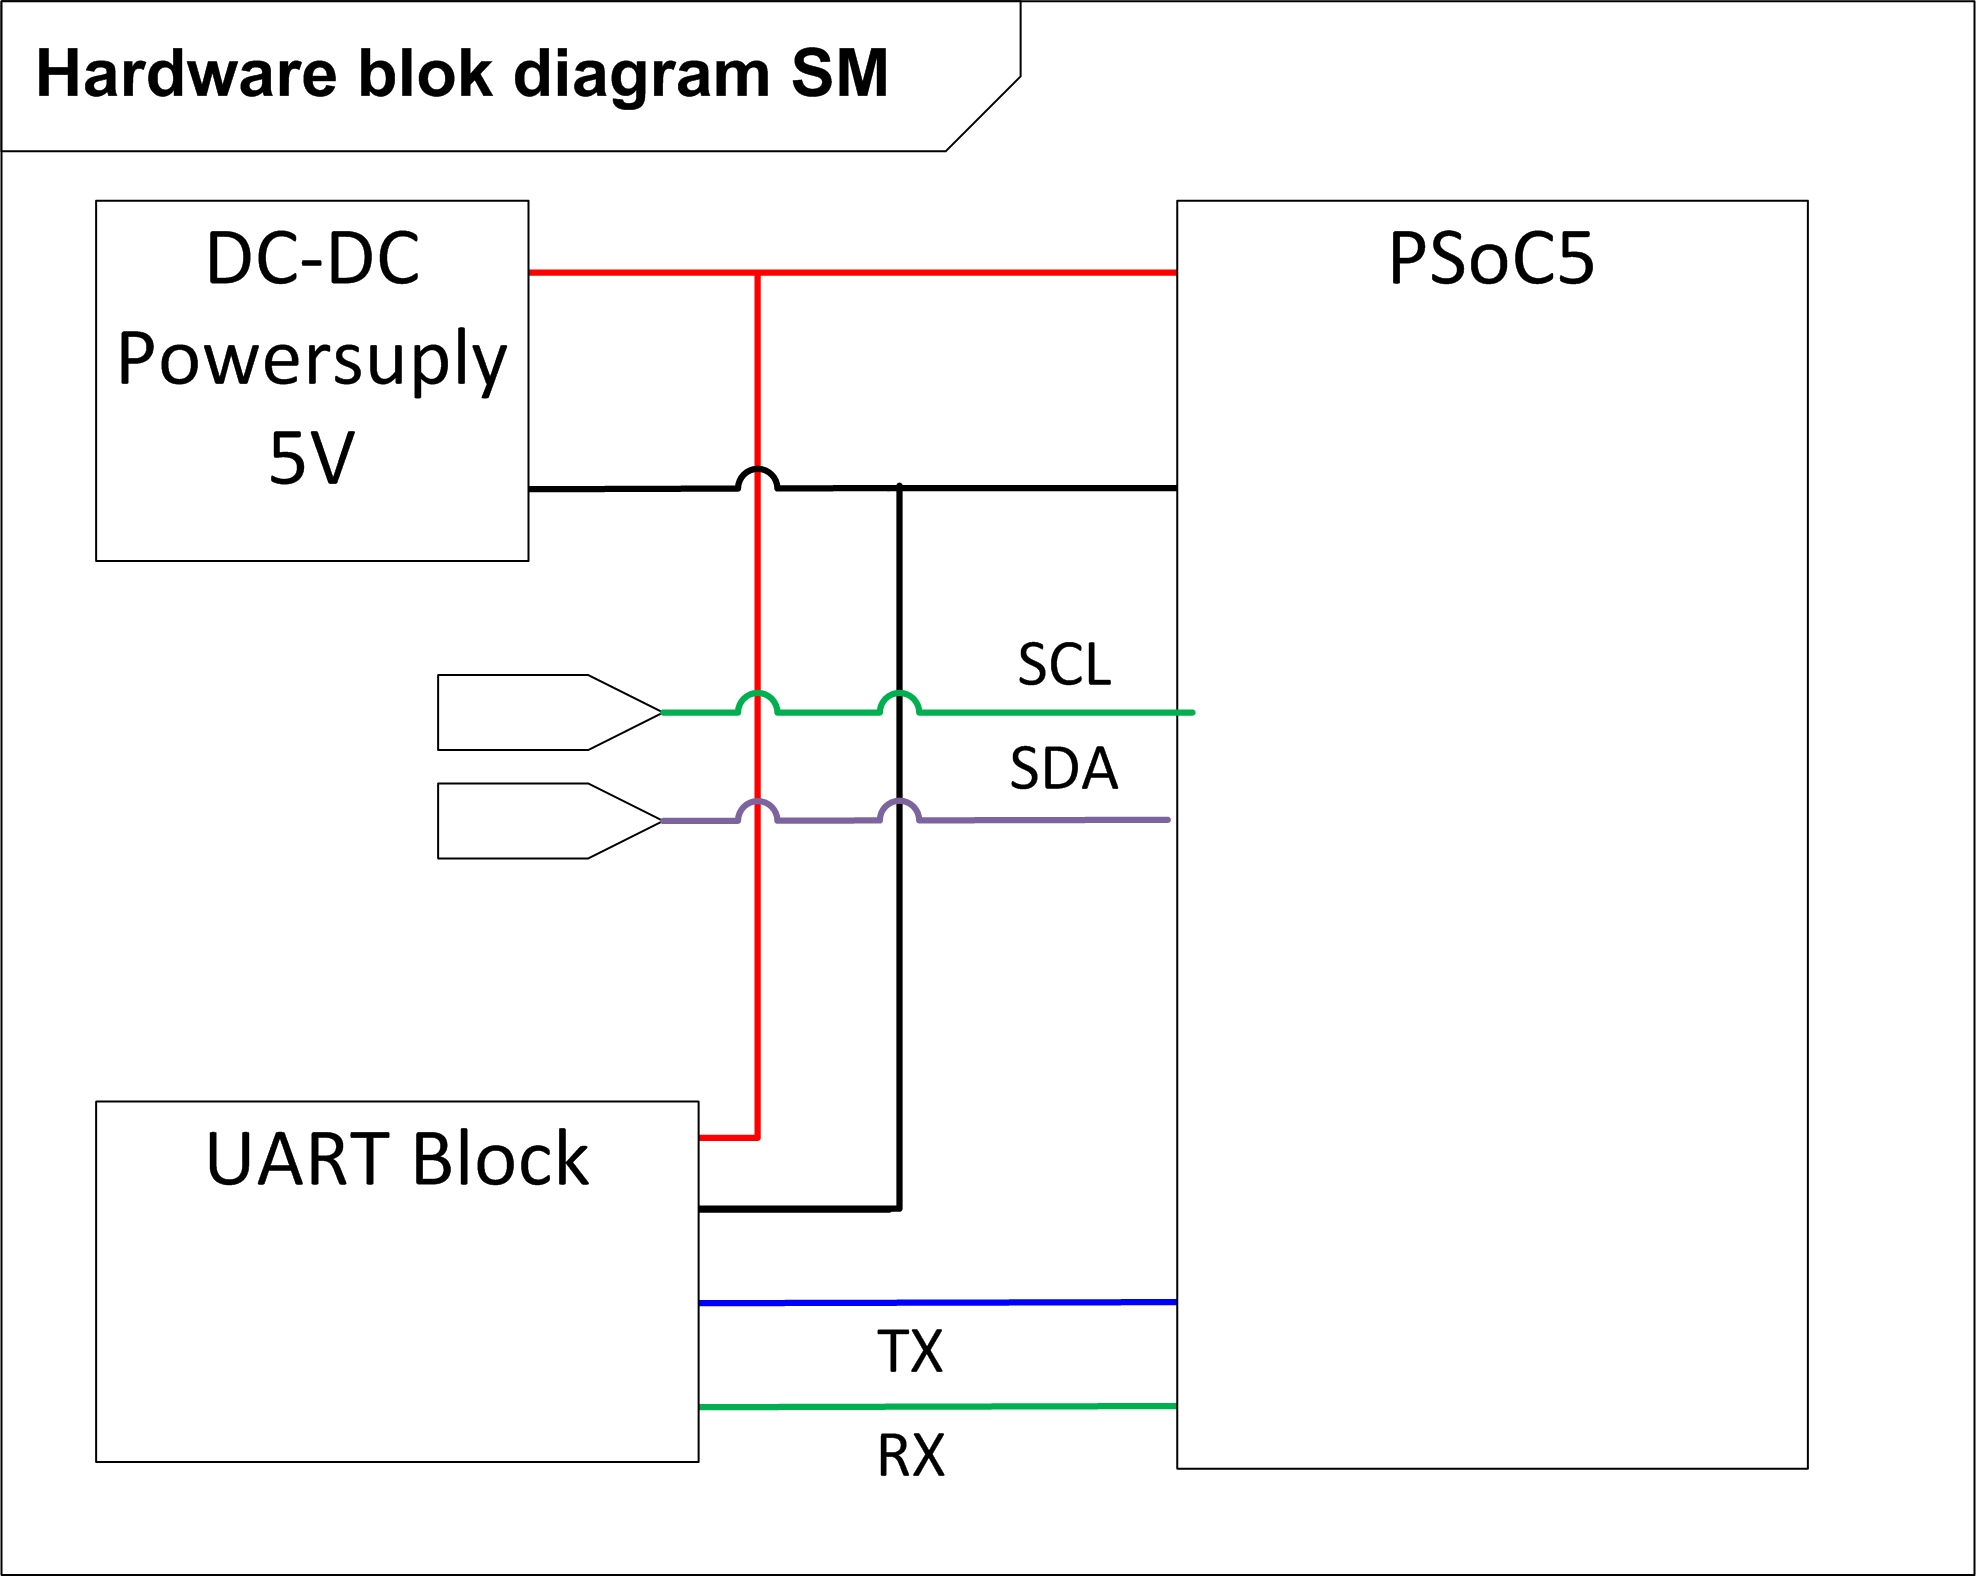
\includegraphics[width=0.5\textwidth]{billeder/SMHardware}
\caption{Overordnet blokdiagram for SM hardware}
\label{fig:HWSM}
\end{figure}
\subsection{Blokke}
Nedenfor beskrives de enkelte blokke illustreret på  \textit{Figur~\ref{fig:HWSM}}.
\subsubsection{PSoC5}
PSoC'en er den centrale del af VBTE'en og står for styringen af hele VBTE'en. Den består af:
\begin{itemize}
\item MicroController
\item I2C
\item Delta-Sigma ADC
\item Accelerometer kontrolregister
\item UART
\end{itemize}
PSoC'en er et færdigkøbt produkt og for detaljer om de enkelte blokke heri henvises der til databladet for PSoC5.
\subsubsection{DC-DC powersuply 5V}
Se powersuply afsnittet.
\subsubsection{UART}
UART-blokken består af en levelkonverter forbundet til et DB9 stik. Levelkonverteren er af typen ST3232.
%%%%%% Nedbrydning af blokke
\section{Nedbrydning af blokke}
Nedenfor følger nedbrydningen af de enkelte blokke med henblik på at designe de enkelte dele til systemet. Nedbrydningen sker for at gøre designet nemmere og mere overskueligt.
\subsection{PSoC5}
På \textit{Figur~\ref{fig:HWPSoCSM}} ses  HW-designet internt på PSoC'en. De enkelte blokke bliver beskrevet efterfølgende.
\begin{figure}[H]
\centering
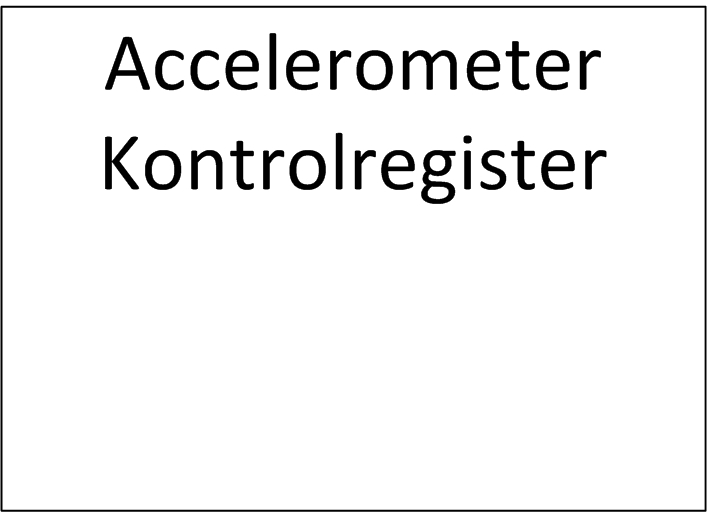
\includegraphics[width=0.7\textwidth]{billeder/SMPSoCblock}
\caption{PSoC5 blokdiagram}
\label{fig:HWPSoCSM}
\end{figure}
\subsubsection{Signalbeskrivelser:}
For signalbeskrivelser se \textit{tabel~\ref{table:PSoCSignalerSM}}
\begin{table}[H]
\begin{tabular}{|p{3cm}|p{3cm}|p{3cm}|p{4.5cm}|} \hline
\cellcolor[gray]{0.85}Signal navn& \cellcolor[gray]{0.85}Type &\cellcolor[gray]{0.85}Spænding&\cellcolor[gray]{0.85}Beskrivelse\\ \hline
TX & Analog & $\sim$0V til $\sim$5V & TX ud til UARTblokken.\\ \hline
RX & Analog & $\sim$0V til $\sim$5V & RX ud til UARTblokken \\ \hline
SDA & Digitalt & $\sim$0V til $\sim$5V & Et digitalt signal mellem VBTE og SM hvor I2C data læses fra.\\ \hline
SCL & Digitalt & $\sim$0V til $\sim$5V & Digitalt clocksignal til I2C.\\ \hline
\end{tabular}
\caption{Tabel over signaler i PSoC blokken}
\label{table:PSoCSignalerSM}
\end{table}
\subsubsection{Blokbeskrivelser:}
\subsubsection{Hældningssensor}
Hældningssensorblokken står for at modtage og konvertere værdier fra hældningssensoren til en integer der er forståelig for vores digitale elektronik. Konverteringen skal se med en A/D konverter med en høj nok opløsning til at måle det udsving angivet i kravspecifikationen.
\subsubsection{UART}
UART kredsen står for at sende og modtage data fra KI. UART operere mellem 0 og 5 volt, og med indstilling sat ud fra \textit{Systemarkitektur/protokoller/UART}. Blocken har 2 signaler der går videre til UART Block, der beskrives senere i dette dokument. 
\subsubsection{Accelerometer Kontrolregister}
Kontrolregisteret står for at sætte indstillinger i vores hældningssensor.
\subsubsection{I2C kreds}
I2C kredsen skal stå for I2C interfacet mellem SM og VBTE. I2C protokollen kører 5V og med pull-up modstande. I2C'en benytter standard I2C protokol, og for yderligere info om data henvises der til \textit{Systemarkitektur/protokoller/I2C}.
%%%%%%%%% UART controller %%%%%%%%%%%%%
\subsection{UART Block}
\begin{figure}[H]
\centering
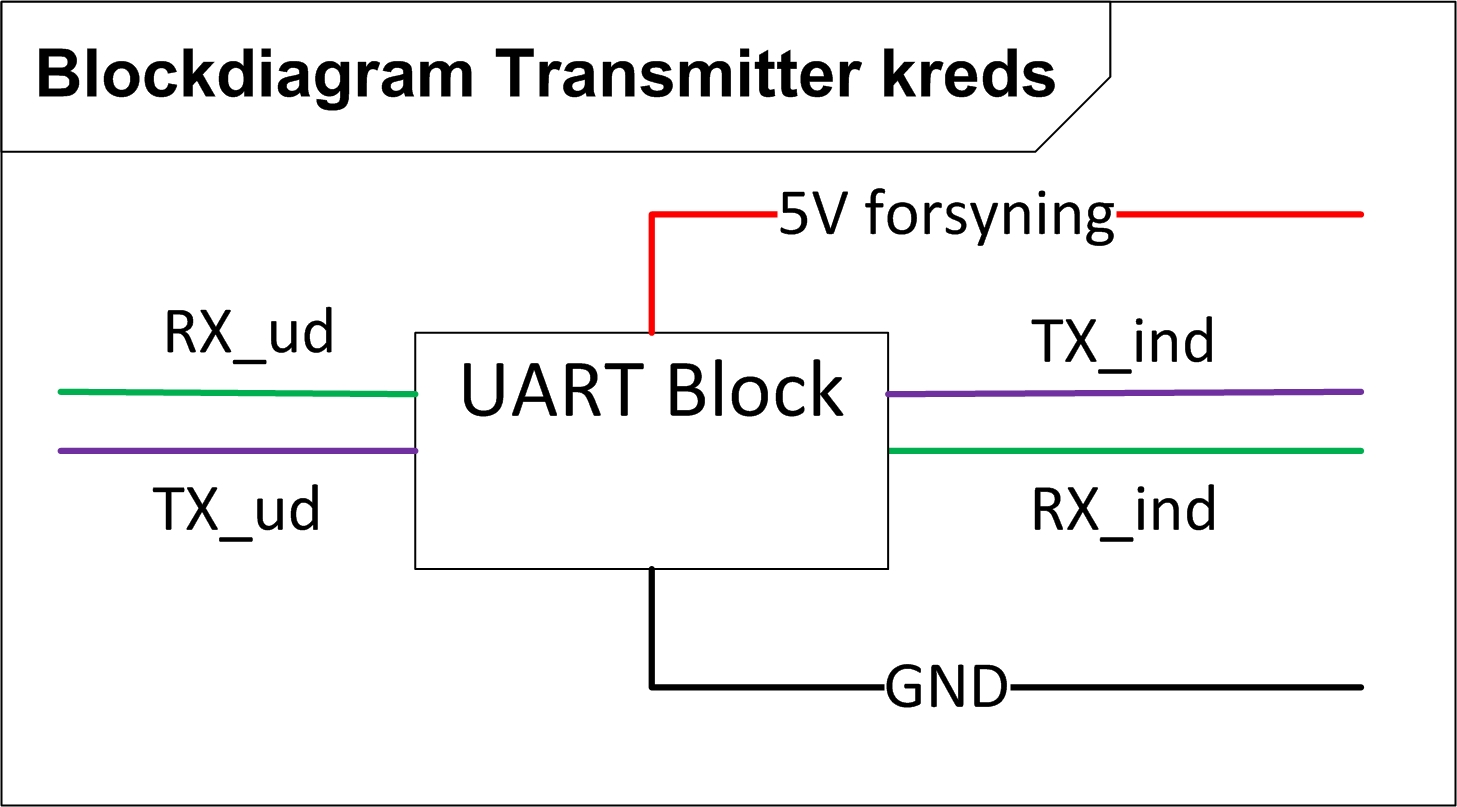
\includegraphics[width=0.5\textwidth]{billeder/uartblock}
\caption{Blokdiagram for Uart Block}
\label{fig:SMUART}
\end{figure}
\subsubsection{Signalbeskrivelser:}
For signalbeskrivelser se \textit{tabel~\ref{table:UARTSignalerSM}}
\begin{table}[H]
\begin{tabular}{|p{3cm}|p{3cm}|p{3cm}|p{4.5cm}|} \hline
\cellcolor[gray]{0.85}Signal navn& \cellcolor[gray]{0.85}Type &\cellcolor[gray]{0.85}Spænding&\cellcolor[gray]{0.85}Beskrivelse\\ \hline
TX\_ud & Analog & $\sim$0V til $\sim$5V & TX fra PSoC blokken.\\ \hline
RX\_ud & Analog & $\sim$0V til $\sim$5V & RX fra PSoC blokken. \\ \hline
TX\_ind & Analog & $\sim$0V til $\sim$5V & TX fra KI modulet.\\ \hline
RX\_ind & Analog & $\sim$0V til $\sim$5V & RX fra KI modulet. \\ \hline
5V forsyning & Analog DC & 5V$\pm$0.1V & 5V forsyning der leveres fra powersupplyen beskrevet under powersupply.\\ \hline
GND & Ground & 0V & Ground i systemet \\ \hline
\end{tabular}
\caption{Tabel over signaler i PSoC blokken}
\label{table:UARTSignalerSM}
\end{table}

%%%%%%%Opbygning af design
\section{Opbygning af design}
Nedenfor følger opbygningen af designet for de forskellige kredse. Dette vl blive beskrevet med Multisim designs, PSoC designs og udregninger. Afsnittet vil starte med at beskrive PSoC designet, da dette er den mest centrale del af SM modulet.
\subsection{PSoC5 design opbygning}
I afsnittet om PSoC'en vil følge 4 underpunkter der beskriver hver blok som illustreret på \textit{Figur~\ref{fig:HWPSoCSM}}.
\subsubsection{Hældningssensor}
\begin{figure}[H]
\centering
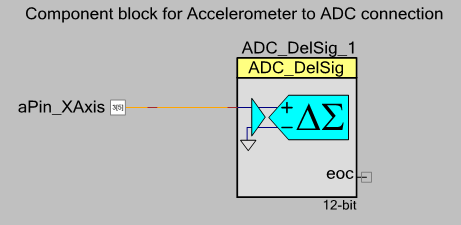
\includegraphics[width=0.7\textwidth]{billeder/levelsensor}
\caption{Realisering for Hældningssensor}
\label{fig:SMLEVEL}
\end{figure}

\subsubsection{UART}
\begin{figure}[H]
\centering
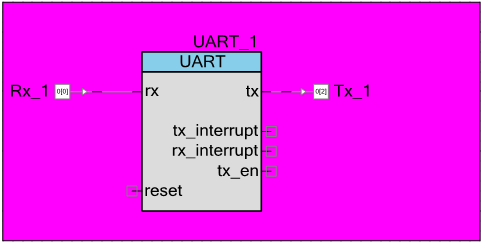
\includegraphics[width=0.7\textwidth]{billeder/uartpsoc}
\caption{Realisering for UART i PSoC}
\label{fig:SMUARTR}
\end{figure}
henning
\subsubsection{Accelerometer Kontrolregister}
\begin{figure}[H]
\centering
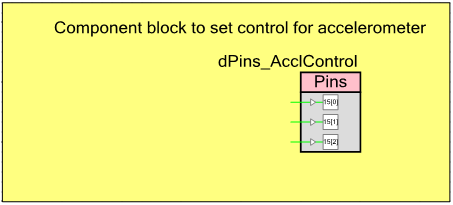
\includegraphics[width=0.7\textwidth]{billeder/Kontrolpsoc}
\caption{Realisering for accelerometer kontrolregister i PSoC}
\label{fig:SMAccReg}
\end{figure}
Accelerometerets kontrolregister sættes ud fra databladet. Fra databladet findes at vi ønsker "ENABLE=1, MODE=1, ST/MODE=LOW". Dette gøres ved sætte registeret til 0x06 eller 0b00000110. Dette giver os den funktionalitet vi søger.
\subsubsection{I2C kreds}
\begin{figure}[H]
\centering
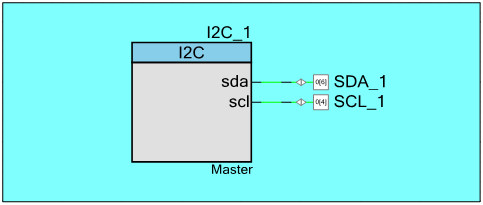
\includegraphics[width=0.7\textwidth]{billeder/i2cpsoc}
\caption{Realisering for i2c i PSoC}
\label{fig:SMi2c}
\end{figure}
I2C realiseres med PSoC'ens indbyggede "Fixed Function" blok hvor vi kører med 100 kbps. Pins sættes via PSoC Creator og resterende funktionalitet styres med software. I softwaren anvendes MasterWriteBuf og MasterReadBuf hvori der anvendes adressen på slaveenheden og arrayet man vil sende. Samtidig er der et indbygget delay så modtageren har tid til at agere på signalet. 
\subsection{UART Block design opbygning}
\textit{Se RS232 Afsnittet}